\chapter{Results \& Discussion}

The algorithms were run in an unmanaged Ubuntu 14.04 cloud server over the course of several weeks. It was found that the algorithms would (somewhat predictably) grow in size as the algorithm narrowed the solution space. This meant that the algorithm's runtime would grow very long. To prevent unreasonably long runtimes, the algorithms were bounded at 6 hours total runtime per graph. Each algorithm was set to test up to 20 times over per graph in the allotted period. The meta-heuristic algorithms are started at their known upper bound, the maximal degree + 1, shown here as $\Delta + 1$, and the number of colours is successively reduced, until the algorithm fails to find a valid colouring.  The successive augmentation algorithm (RBB) does not have a set start position, since it simply tries to find a better valid colouring upon every iteration. Its initial best colouring uses \emph{infinite} colours, and therefore must be lowered upon the first iteration.

\section{Algorithms}
The algorithm are run on 5 graphs of varying difficulty. Sample graphs\footnote{provided for the 1992-1992 DIMACS Implementation Challange for NP-Hard Problems: Max Clique, Graph Coloring, and SAT.} were run successively for each algorithm up to 20 times, the average time to the given colouring, and the success rate for each algorithm to attain that colouring is shown in Table \ref{res:timeToK}. The total runtimes for each algorithm are shown in Table \ref{res:timeToFail}, signifying the amount of time that the algorithm required to not find a better solution. Note that due to the hard limitation of 6 hours (21600 seconds) on each algorithm, better colourings may have been attained had the algorithm been allowed to run for a longer amount of time. 
\begin{table}[H]
\label{results1}
\centering
\begin{tabular}{|l c c l c c c|}
\hline
Graph & $\chi$ & $\Delta + 1$ & Solver & k & avg time to k (sec)& \% success\\ \hline

myciel4.col    & 5  & 12  & RBB & 5 & 0 & 100\\
myciel4.col    & 5  & 12  & GS  & 5 & 0.05 & 100\\
myciel4.col    & 5  & 12  & FPA & 5 & 0.9 & 100\\
myciel4.col    & 5  & 12  & GA  & 5 & 24.7 & 100\\ \hline

queen5\_5.col  & 5  & 17  & RBB & 5 & 0.001 & 100\\
queen5\_5.col  & 5  & 17  & GS  & 5 & 1.27 & 100\\
queen5\_5.col  & 5  & 17  & FPA & 9 & 113.4 & 80\\
queen5\_5.col  & 5  & 17  & FPA & 10 & 36.2 & 100\\
queen5\_5.col  & 5  & 17  & GA  & 5 & 3984.5 & 12\\
queen5\_5.col  & 5  & 17  & GA  & 6 & 218.4 & 63\\ \hline

myciel5.col    & 6  & 24  & RBB & 6 & 0.001 & 100\\
myciel5.col    & 6  & 24  & GS  & 6 & 0.8 & 100\\
myciel5.col    & 6  & 24  & FPA & 8 & 1918.5 & 13\\
myciel5.col    & 6  & 24  & FPA & 8 & 464.4 & 93\\
myciel5.col    & 6  & 24  & GA  & 6 & 12814.1 & 100\\ \hline

queen7\_7.col  & 7  & 25  & RBB & 7 & 0.7 & 5\\
queen7\_7.col  & 7  & 25  & RBB & 8 & 0.5 & 75\\
queen7\_7.col  & 7  & 25  & GS  & 9 & 678.5 & 5\\
queen7\_7.col  & 7  & 25  & GS  & 19 & 42.2 & 100\\
queen7\_7.col  & 7  & 25  & FPA & 20 & 2483.2 & 60\\
queen7\_7.col  & 7  & 25  & FPA & 21 & 887.1 & 100\\
queen7\_7.col  & 7  & 25  & GA  & 14 & 5089.4 & 100\\ \hline

mulsol.i.3.col & 31 & 158 & RBB & 31 & 0.001 & 100\\
mulsol.i.3.col & 31 & 158 & GS  & 31 & 5397 & 10\\
mulsol.i.3.col & 31 & 158 & GS  & 32 & 2815.5 & 50\\
mulsol.i.3.col & 31 & 158 & GS  & 33 & 1944.5 & 100\\
mulsol.i.3.col & 31 & 158 & FPA & 81 & 21083.8 & 50\\
mulsol.i.3.col & 31 & 158 & FPA & 82 & 3585.5 & 100\\
mulsol.i.3.col & 31 & 158 & GA  & 82 & 19960.3 & 100\\ \hline
\end{tabular}
\caption{Results showing the time taken for the algorithm to find a valid colouring (k colours), optimal or not}
\label{res:timeToK}
\end{table}

\begin{table}[H]
\label{results2}
\centering
\begin{tabular}{|l c c l c c|}
\hline
Graph & $\chi$ & $\Delta + 1$ & Solver & min k reached & total runtime (sec) \\\hline

myciel4.col    & 5  & 12  & RBB & 5 & 0.47\\
myciel4.col    & 5  & 12  & GS  & 5 & 161.9\\
myciel4.col    & 5  & 12  & FPA & 5 & 225.7\\
myciel4.col    & 5  & 12  & GA  & 5 & 173.5\\ \hline

queen5\_5.col  & 5  & 17  & RBB & 5 & 0.3\\
queen5\_5.col  & 5  & 17  & GS  & 5 & 388.5\\
queen5\_5.col  & 5  & 17  & FPA & 9 & 496.6\\
queen5\_5.col  & 5  & 17  & GA  & 5 & 21600$^\star$\\ \hline

myciel5.col    & 6  & 24  & RBB & 6 & 1.3\\
myciel5.col    & 6  & 24  & GS  & 6 & 512.6\\
myciel5.col    & 6  & 24  & FPA & 8 & 2929.4\\
myciel5.col    & 6  & 24  & GA  & 8 & 21600$^\star$\\ \hline

queen7\_7.col  & 7  & 25  & RBB & 7 & 1.1\\
queen7\_7.col  & 7  & 25  & GS  & 9 & 1795.3\\
queen7\_7.col  & 7  & 25  & FPA & 20 & 4806.5\\
queen7\_7.col  & 7  & 25  & GA  & 15 & 21600$^\star$\\ \hline

mulsol.i.3.col & 31 & 158 & RBB & 31 & 19.05\\
mulsol.i.3.col & 31 & 158 & GS  & 31 & 7972.9\\
mulsol.i.3.col & 31 & 158 & FPA & 81 & 21600$^\star$\\
mulsol.i.3.col & 31 & 158 & GA  & 82 & 21600$^\star$\\ \hline
\end{tabular}
\caption{Results of algorithms attempts at finding a better solution (and failing)}
\label{res:timeToFail}
\end{table}

It is interesting to note that the successive augmentation algorithm RBB does not exhibit a blowup in time when it gets close to a solution, indeed it actually \emph{speeds up} as it narrows its scope. It exhibits a polynomial dependence on the number of vertices a graph contains. However it is not guaranteed to converge to the optimal solution, even after infinitely many iterations. The meta-heuristic algorithms are seen to get dramatically slower with the addition of more vertices, and are also affected by the narrowing of the search space. The FPA and GA were especially affected by the narrowing of the search space, each hitting the time limit upon their iterations well before reaching the optimal solution. The GS does not suffer from this problem to such an extreme degree, but the time taken does increase dramatically as the solution space narrows.

Each solver was seen to struggle when faced with graphs with a complex geometry. For these graphs, like the hypercube-class graphs which are bipartite by design, all algorithms were seen to struggle obtaining a solution due to the highly ordered structure of the underlying problem.

Note that the runtimes marked ($^\star$) were terminated at maximal runtime, and a better solution may have been found had the algorithm been allowed to continue.

\begin{figure}[H]
\caption{Asymptotic runtime for graph mulsol.i.3. Blue: GS, Red: FPA, Green: GA}
\centering
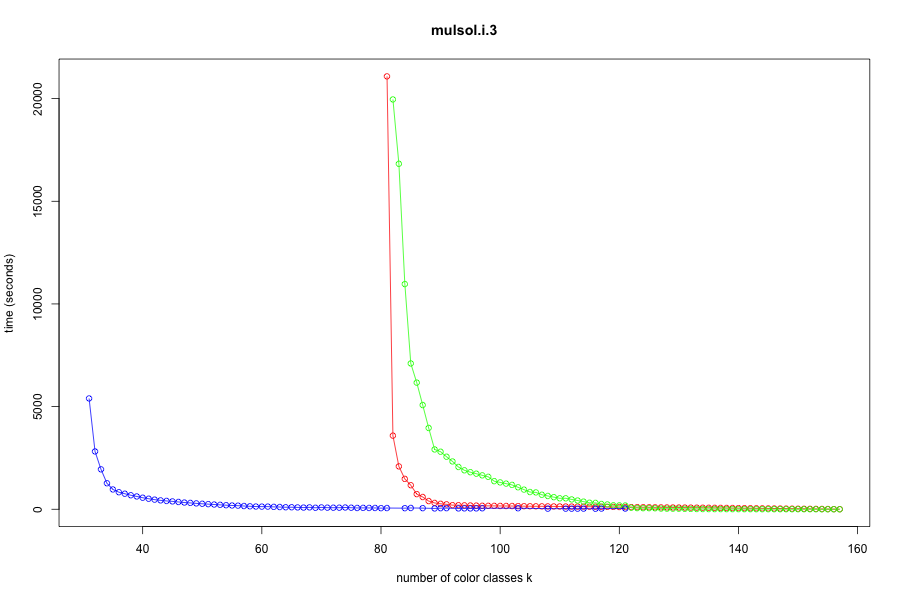
\includegraphics[height=0.4\textheight]{a1-mulsol-i-3-col}
\end{figure}

\begin{figure}[H]
\caption{Asymptotic runtime for graph mulsol.i.3. Blue: GS, Red: FPA, Green: GA}
\centering
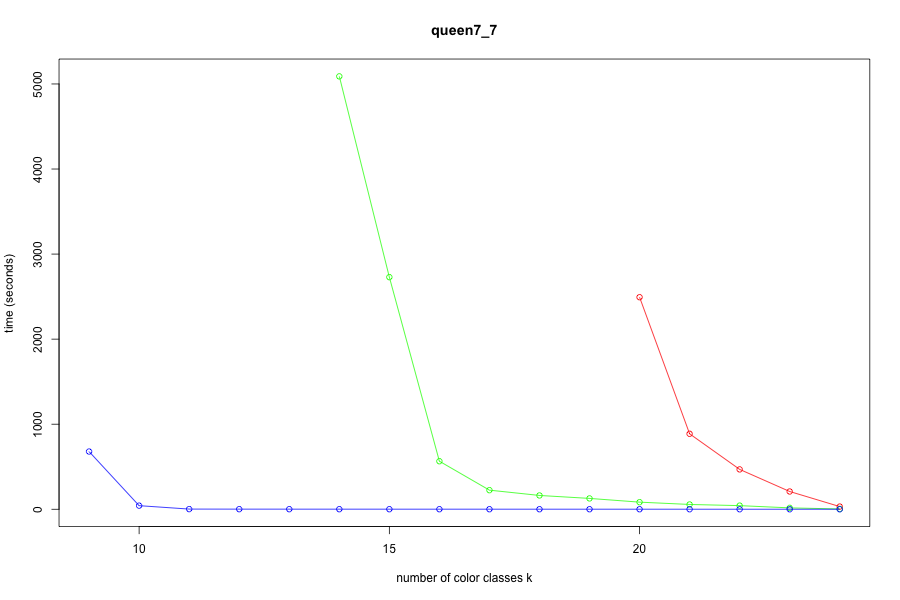
\includegraphics[height=0.4\textheight]{a5-queen7_7-col}
\end{figure}

So pretty!

